% \section{Visualization design}
% \subsection{Query execution overview}
% \subsubsection{Execution plan view}
% \subsubsection{Execution progress view}
% \subsection{Task view}
% \subsection{System profiling visualization}
% \subsection{Linkage and interactions}

\section{Visualization Design}

<<<<<<< HEAD
=======
Following the data modeling, we present our web-based visual analytics system $\DQV$, which supports interactive exploration of the query execution process with four coordinated views. The \textit{execution progress} demonstrates an overview about how the query plan is executed (\textbf{T1}), the \textit{task distribution view} shows the task distribution and their data dependencies. Integrated with the performance statistics of the machines, this view also help reason the system causes of task performance (\textbf{T2} and \textbf{T3}). \textit{Task list} provides detailed information of individual tasks (\textbf{T2}).  At last, interaction and linkage are introduced to support multi-level exploration (\textbf{T4}).

>>>>>>> 87e38476d46c232532b1981a1ff0ea0f46d2299d
\subsection{Query Progress View}\label{sec:queryprogress}


\begin{figure}[t]
	\centering
	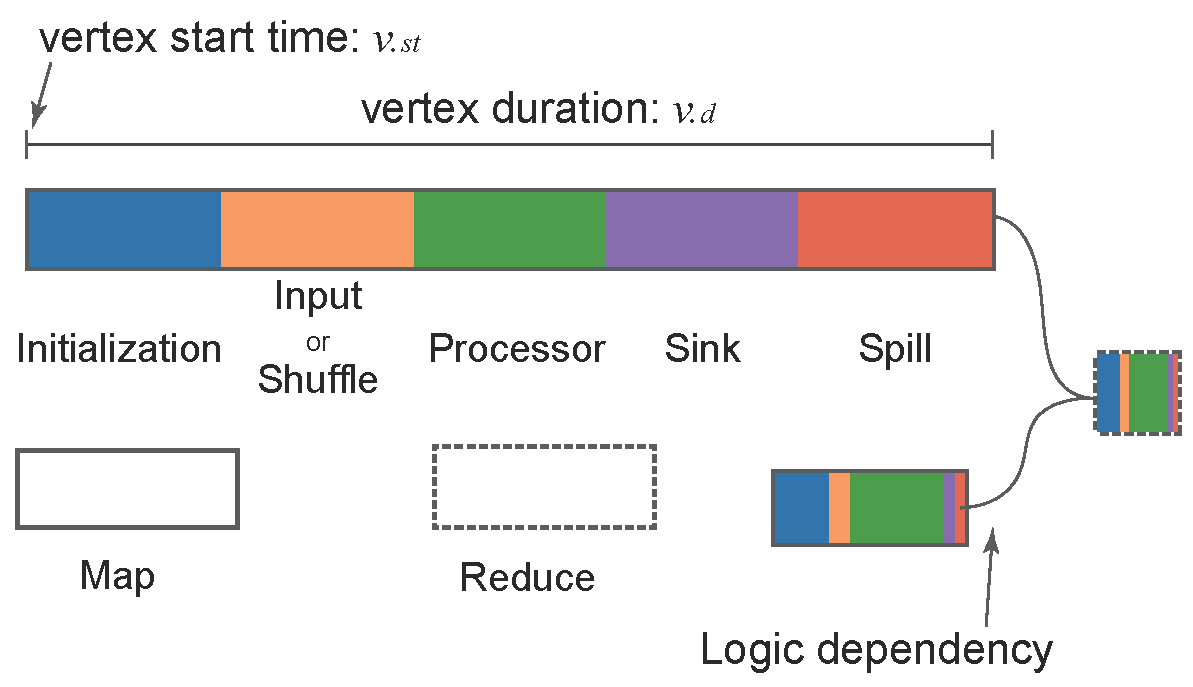
\includegraphics[width=0.35\textwidth]{figures/visualization/progressdesign.pdf}
	\vspace{-3mm}
	\caption{Visual encoding of logic vertex and dependencies}
	\label{fig:progress}
	\vspace{-3mm}
\end{figure}

<<<<<<< HEAD
Query Progress View is developed to overview the overall progress of query execution and the logic dependencies. 

\begin{algorithm}
	\caption{$\mathsf{TDAGLayout}$($R$, $canvas$)}
	\label{alg:TDAGLayout}
	\begin{algorithmic}[1]
		\For {$root$ in $R$}
		\State$\mathsf{process}$($root$, $canvas$)
		\EndFor
	\end{algorithmic}

\end{algorithm}

\begin{algorithm}
	\caption{$\mathsf{process}$($v$, $canvas$)}
	\label{alg:process}
	\begin{algorithmic}[1]
		\If{$v.visit = True$}
			\State Do Nothing
		\EndIf
		\If{$v.children$ is empty}
			\If{$\mathsf{place}$($v$)$ = true $}
				\State $canvas.height \leftarrow canvas.height + uh$
				\State $\mathsf{place}$($v$)
			\EndIf
		\Else
			\For {$c$ in $v.children$}
				\State $\mathsf{process}$($c$)
				\If{$\mathsf{place}$($v$)$ = true$}
					\State $v.visit \leftarrow True$
				\EndIf
			\EndFor
			\If{$v.visit = True$}
				\State $canvas.height \leftarrow canvas.height + uh$
				\State $\mathsf{place}$($v$)
			\EndIf
		\EndIf
	\end{algorithmic}
\end{algorithm}




\subsubsection{Visual Encoding}
The commonly used method to visualize the progress data is Gantt Chart.
As shown by Figure~\ref{fig:progress}, the x-axis indicates the timestamp. The rectangles with the same height indicate the temporal information of logic vertices. 
Given a vertex $v$, the position of the left side indicates the start time $v.st$ and the duration of $v.d$ is encoded by the length of the rectangle. We use the stroke dash to present the type of vertex and use the color to encode the type of steps in a vertex. Moreover, the order of all steps is fixed as shown by Figure~\ref{fig:progress}.

\subsubsection{Layout Method}
In Gantt Diagram has been deployed to many progress visualization tools such as Tez UI and Tabula, each progress bar takes up the whole line with its left side and length encode the start time and duration, which is shown as Figure~\ref{fig:layout}(A).
Vertically, the progress bars are ordered by the start time of the vertex. In this visual design, since the layout doesn't consider the logic dependencies, it always results in a very serious cross between the links and unclear topology structure.

To tackle this problem, we design an algorithm~\ref{alg:TDAGLayout} to layout the TDAG. With an edge $e=\{u,v\}$, we define $u$ as the child of $v$ and $v$ as the parent of $u$. Moreover, we define the $root$ as the vertex which has no parents. $\mathsf{process}$ is described as Algorithm~\ref{alg:process}, which use a in-order traversal to process the vertices in the graph.  $\mathsf{place}$ is the function which tries to place the vertex in the canvas. At first, we use a naive which provides a vertex an exclusive row, which is shown as Figure~\ref{fig:layout}(B). The new layout shows a clear topology structure because the brother vertices are visited closely. However, this methods also results in a poorly using of the canvas, since some vertices can be put at the same row.  
To provide a tight layout, we revise the method $\mathsf{place}$ which tries to place the vertex at the top position of the canvas, if the vertex is overlaped with the existing vertex, then move this vertex down the distance of the vertex height. If the $\mathsf{place}$ cannot find a place for the vertex in the canvas, the $\mathsf{place}$ will return $False$ indicating the height of canvas is not enough, otherwise return $True$. Each parent vertex will be visited multiple times until it is successfully placed into the canvas(shown as line 10 to line 14). The result(Figure~\ref{fig:layout}(B)) shows a layout which requires a smaller canvas.

The tight layout further results in an unclear structure of the dependencies. We further optimized it by changing the position of the control points of B-splines. With two different source vertex, the x-position of the control points are different, thus making the lines from different source vertices are attracted to different position. The results is shown as Figure~\ref{fig:layout}(D).
=======
Query progress view is developed to show the overall progress of query execution and the logical dependencies among the operators. 

\begin{algorithm}
	\caption{$\mathsf{TDAGLayout}$ ($R$, $canvas$)}
	\label{alg:TDAGLayout}
	\begin{algorithmic}[1]
		\For {$root$ in $R$}
		\State$\mathsf{process}$($root$, $canvas$)
		\EndFor
	\end{algorithmic}

\end{algorithm}

\begin{algorithm}
	\caption{$\mathsf{process}$($v$, $canvas$)}
	\label{alg:process}
	\begin{algorithmic}[1]
		\If{$v.visit = True$}
			\State Do Nothing
		\EndIf
		\If{$v.children$ is empty}
			\If{$\mathsf{place}$($v$)$ = true $}
				\State $canvas.height \leftarrow canvas.height + uh$
				\State $\mathsf{place}$($v$)
			\EndIf
		\Else
			\For {$c$ in $v.children$}
				\State $\mathsf{process}$($c$)
				\If{$\mathsf{place}$($v$)$ = true$}
					\State $v.visit \leftarrow True$
				\EndIf
			\EndFor
			\If{$v.visit = True$}
				\State $canvas.height \leftarrow canvas.height + uh$
				\State $\mathsf{place}$($v$)
			\EndIf
		\EndIf
	\end{algorithmic}
\end{algorithm}


\subsubsection{Visual Encoding}
%The traditional method to visualize the progress data is the Gantt Chart~\cite{clark1922gantt} which maps the time interval on the horizontal axis and lists the progresses bar on the vertical axis.
%As shown by Figure~\ref{fig:progress}, given a vertex $v$, the x-coordinate of the bar's left side indicates the start time $v.st$ and the duration of $v.d$ is encoded by the length of the rectangle. We use the stroke dash to present the type of vertex and use the color to encode the type of steps in a vertex. Moreover, the order of all steps is fixed as shown by Figure~\ref{fig:progress}, and we use B-splines to show the dependencies.

The Gantt Chart~\cite{clark1922gantt} is widely used to visualize progress data, which maps the time interval to the horizontal axis and lists the progress bars on the vertical axis.
As shown in Figure~\ref{fig:progress}, for a vertex $v$ in the logical execution plan, the leftmost x-coordinate of its bar indicates the start time $v.st$ and its duration $v.d$ is encoded by the length of the bar. We use stroke and dash to represent the type of vertex (i.e., map or reduce) and adopt different colors to encode the sub-steps of a vertex. Note that the order of the sub-steps is fixed as shown by Figure~\ref{fig:progress}. We use B-splines to show the dependencies among the tasks.

\subsubsection{Layout Method}
%Gantt Chart has been used in many progress visualization tools such as Tez UI and Tabula, in which each progress bar takes up the whole line, which is shown as Figure~\ref{fig:layout}(A).
%Vertically, the progress bars are ordered by the start time of the vertex. In this visual design, since the layout doesn't consider the logic dependencies, it always has a very serious cross between the links and unclear topology structure.
%
%To tackle this problem, we design an algorithm~\ref{alg:TDAGLayout} to layout the TDAG. Notice that since the x-position and width of the bars have been fixed to encode the temporal information, only the vertical position can be changed to optimize the layout. With an edge $e=\{u,v\}$, we define $u$ as the child of $v$ and $v$ as the parent of $u$. Moreover, we define the $root$ as the vertex which has no parents. $\mathsf{process}$ is described as Algorithm~\ref{alg:process}, which use a in-order traversal to process the vertices in the graph.  $\mathsf{place}$ is the function which tries to place the vertex in the canvas. At first, we use a naive which provides a vertex an exclusive row, which is shown as Figure~\ref{fig:layout}(B). The new layout shows a clear topology structure because the brother vertices are visited closely. However, this method also results in a poorly using of the canvas because each vertex will take the whole row.  
%
%To provide a tight layout, we revise the method $\mathsf{place}$ which tries to place the vertex at the top position of the canvas, if the vertex is overlapped with the existing vertex, then move this vertex down the distance of the vertex height. If the $\mathsf{place}$ cannot find a place for the vertex in the canvas, the $\mathsf{place}$ will return $False$ indicating the height of canvas is not enough, otherwise return $True$. Each parent vertex will be visited multiple times until it is successfully placed into the canvas(shown as line 10 to line 14). The result(Figure~\ref{fig:layout}(C)) shows a layout which requires a smaller canvas than Figure~\ref{fig:layout}(B).
%
%The tight layout further results in an unclear structure of the dependencies because it compress the space to put the links. We further optimized it by changing the position of the control points of B-splines. With two different source vertex, the x-position of the control points are different, thus making the links from different source vertices are attracted to different position. The result is shown as Figure~\ref{fig:layout}(D).


The Gantt chart has been used in many progress visualization tools such as Tez UI and Tabula, in which each progress bar takes up an entire line as shown in Figure~\ref{fig:layout}(A). Vertically, the progress bars are ordered by the start time of the corresponding vertices. In existing visual design, the layout doesn't consider the logical dependencies among the vertices, which results in many cross edges and fails to show a clear topology structure.


To tackle this problem, we design Algorithm~\ref{alg:TDAGLayout} to layout the TDAG. As the horizontal position and width of the bars are used to encode temporal information, only the vertical position can be adjusted to optimize the layout. For an edge $e=\{u,v\}$, we define $u$ as the child of $v$ and $v$ as the parent of $u$. Moreover, we define the $root$ of a TDAG as the vertex which has no parents. As described in Algorithm~\ref{alg:process}, $\mathsf{process}$ uses an in-order traversal to process the vertices in the TDAG, in which $\mathsf{place}$ is a function that tries to place a vertex in the canvas. At first, we follow the naive approach and place each vertex in an exclusive row. As shown in Figure~\ref{fig:layout}(B), the layout shows a clearer topology structure compared with Figure~\ref{fig:layout}(A) as the sibling vertices are placed close to each other. However, this method requires a large canvas because each vertex takes up a row, which will result in serious scalability problem when the TDAG contains many vertices.  

To provide a tight layout, we revise the $\mathsf{place}$ method by trying to place each vertex at the top of the canvas. If a vertex overlaps with an existing vertex, then we move this vertex down by the width of a bar $uh$. If $\mathsf{place}$ cannot find a position for the vertex in the canvas, it returns $false$ indicating that the height of the canvas is not enough. Each parent vertex will be visited multiple times until it is successfully placed into the canvas (line 10~14 in Algorithm~\ref{alg:TDAGLayout}). As shown in Figure~\ref{fig:layout}(C), this layout requires a smaller canvas than Figure~\ref{fig:layout}(B). However, the tight layout does not show a clear dependency structure as it compress the space to put the links and creates many cross links. Therefore, we further optimize the placement method by  changing the position of the control points of the B-splines. For two different source vertices, the x-positions of their control points are different, which enables the links from different source vertices to attach to different positions. The result is shown in Figure~\ref{fig:layout}(D).
>>>>>>> 87e38476d46c232532b1981a1ff0ea0f46d2299d

\begin{figure}[t]
	\centering
	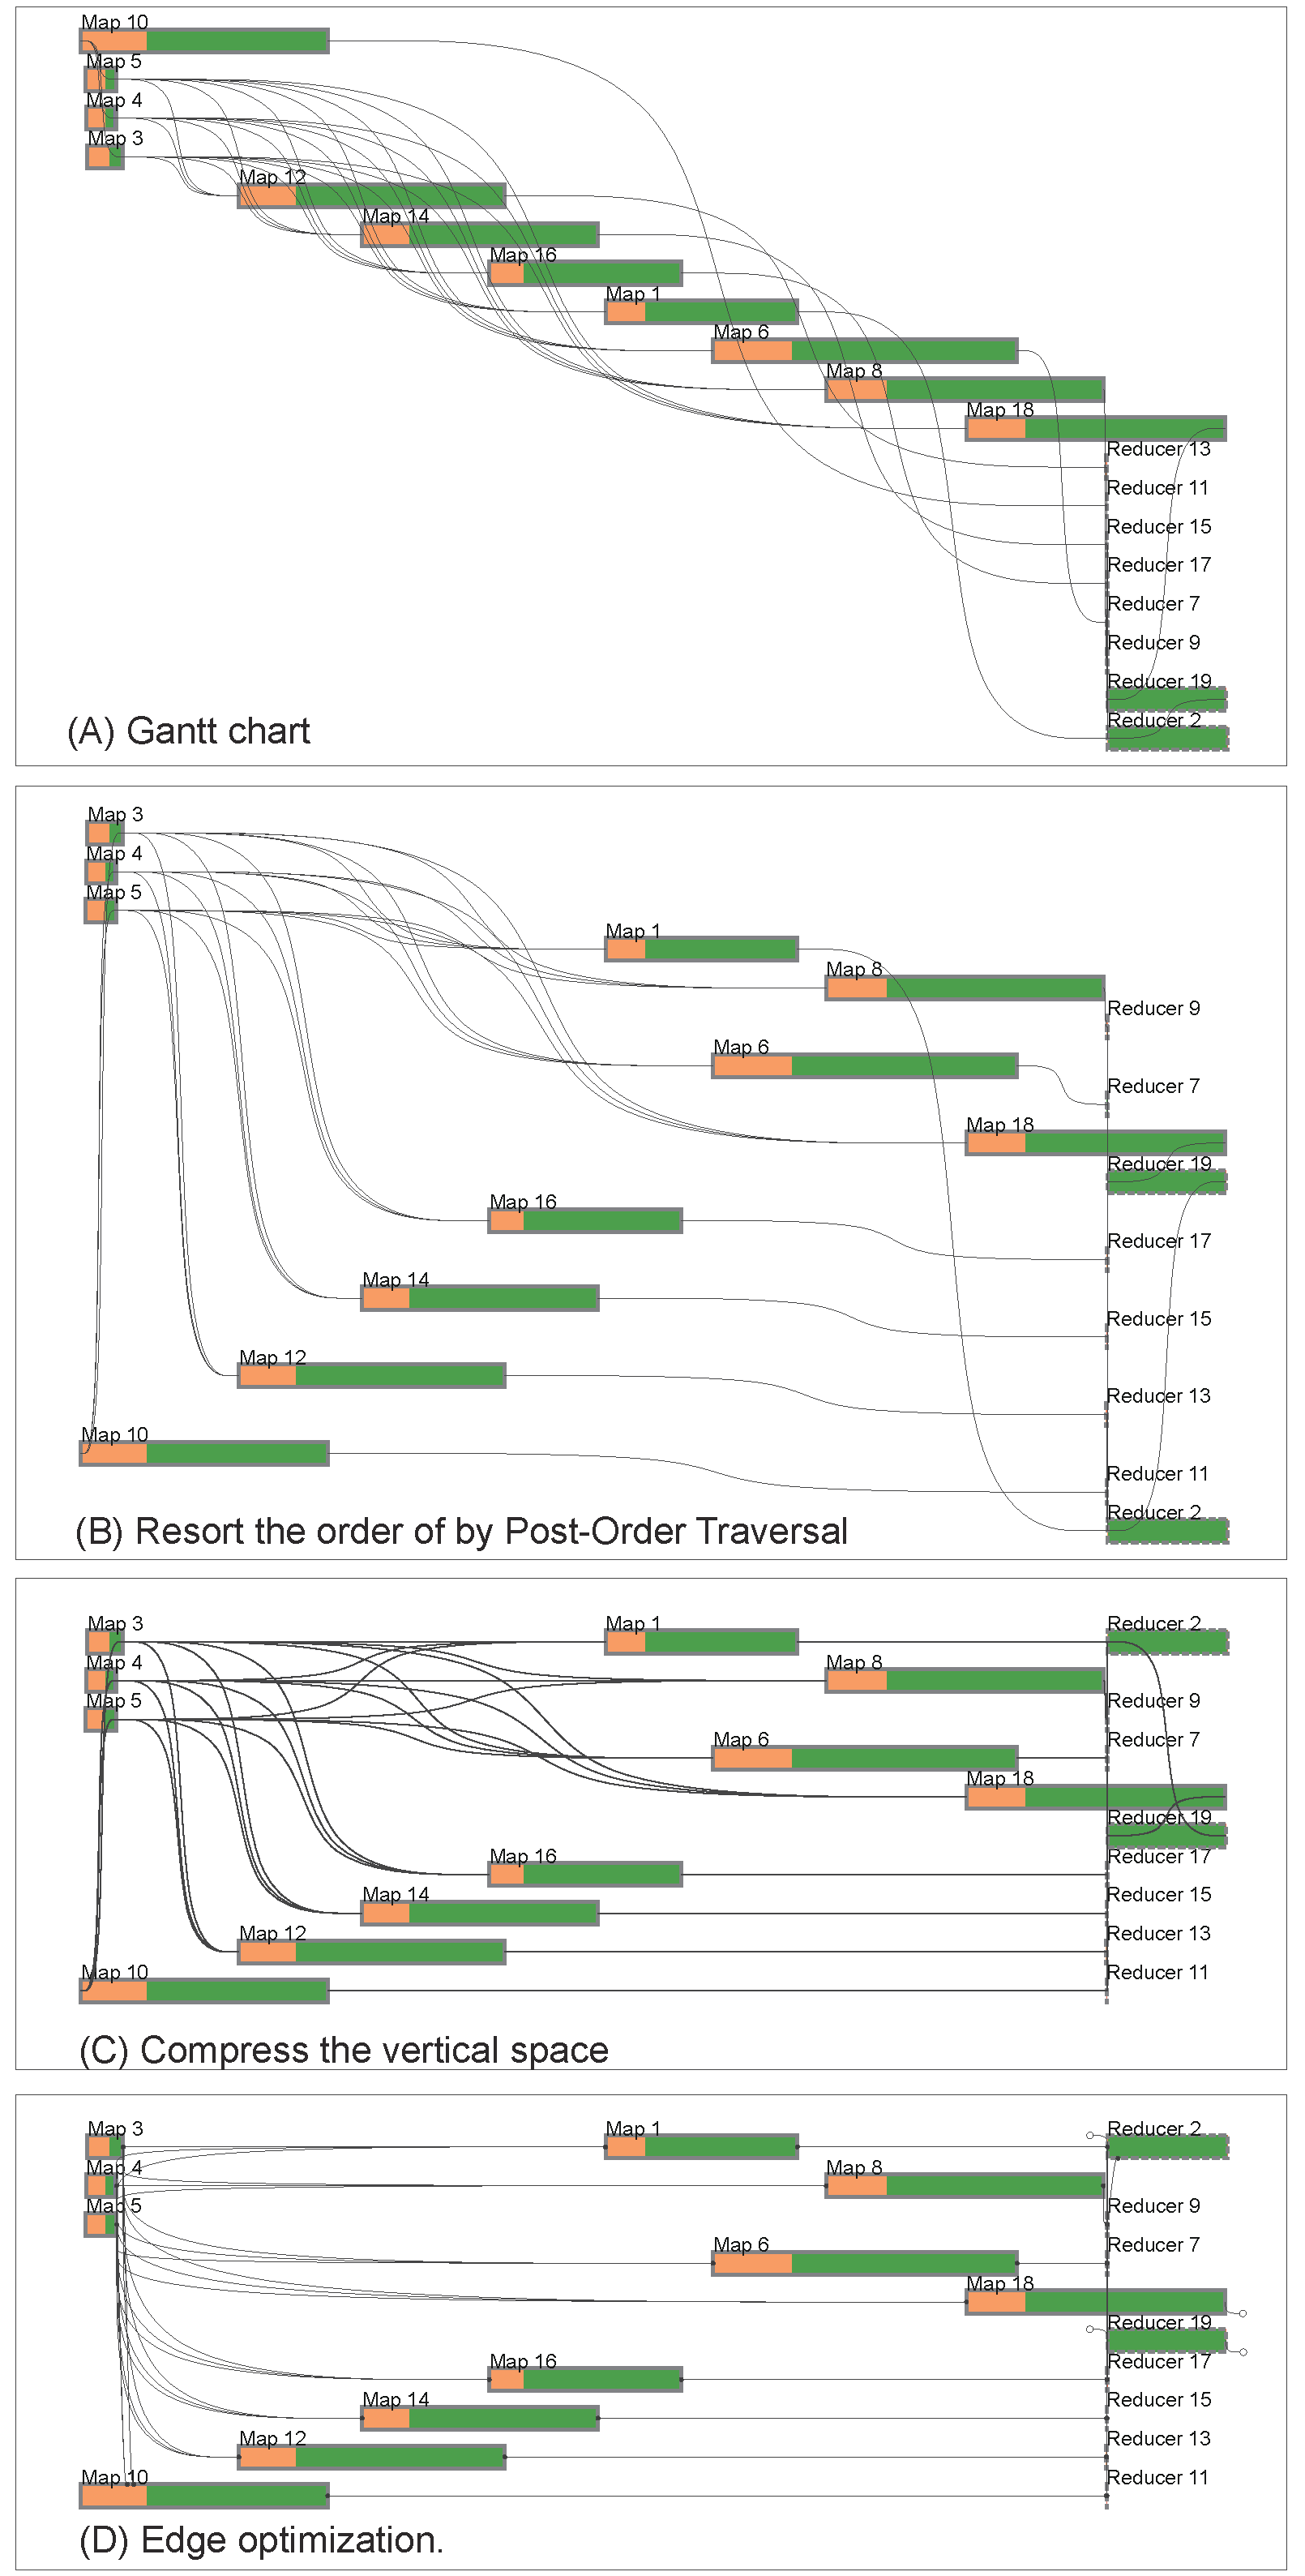
\includegraphics[width=0.45\textwidth]{figures/visualization/exeprogress.pdf}
	\vspace{-3mm}
	\caption{Temporal DAG layout algorithms}
	\label{fig:layout}
	\vspace{-3mm}
\end{figure}
%\begin{itemize}
%    \item Traditional method: Gantt diagram and design consideration 
%    \item Proposed algorithms, link processing
%    \item Alternative design
%        \begin{itemize}
%            \item Gantt(consider the vertical edge, large space, unclear structure)
%            \item New design loose(clear structure, large space)
%            \item New design compact(small space, unclear structure    )
%        \end{itemize}
%\end{itemize}

% -Visual form of Gantt diagram
% -Our design consideration
% -Algorithms
% -Design alternatives
% --gantt(consider the vertical edge, large space, unclear structure)
% --new design loose(clear structure, large space)
% --new design compact(small space, unclear structure)
% --new design compact, edge processing(small space, clear structure)
\subsection{Pattern Explorer}


\begin{figure}[t]
	\centering
	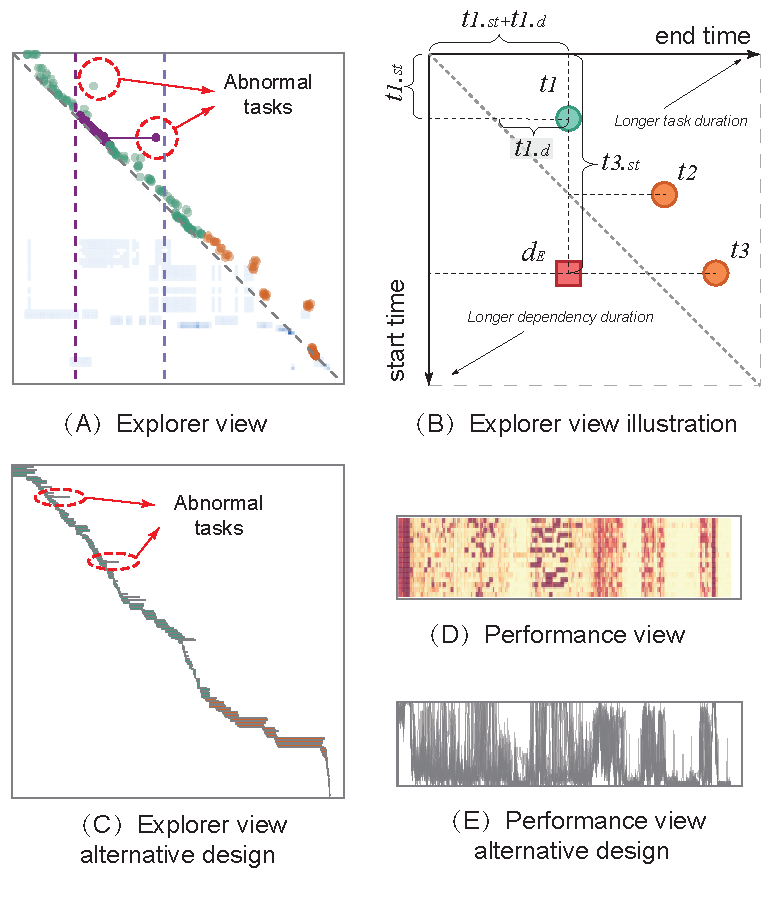
\includegraphics[width=0.48\textwidth]{figures/visualization/patternexplorer.pdf}
	\vspace{-3mm}
	\caption{Visual design for the pattern explorer.}
	\label{fig:explorer}
	\vspace{-3mm}
\end{figure}


<<<<<<< HEAD
Pattern Explorer is developed to provide efficient pattern discovery and reasoning at the task-level. This component consists of multiple coordinated views, including Distribution View and Performance View.
\subsubsection{Distribution View}
The Distribution View is designed to explore the temporal pattern and dependencies of tasks.

\stitle{Visualizing the temporal information of tasks}
Before our collaboration, the domain experts use Gantt Chart Diagram to display the overall progress of tasks, shown in figure~\ref{fig:explorer}(C). 
However, Gantt Chart Diagram-based method suffers significant scalability problem in our applications. Hundreds to thousands of tasks are associated with a vertex in our scenario, which requires a very large space to place all the horizontal bars clearly. 
Moreover, visualizing a large number of bars in this way is difficult for users to compare the absolute length of the horizontal bars due to the lack of alignment, which hinders the users' ability to discover the group-based patterns or identify the abnormal tasks.

To tackle this issue, we develop a scatter-based visual representation which is shown as Figure~\ref{fig:explorer}(A). Figure~\ref{fig:explorer}(B) illustrates the visualization design which uses a square shape of rendering canvas as the basis, the vertical axis(from top to bottom) indicates the start time, and the horizontal axis(from left to right) indicates the end time.
The task(e.g., $t_1, t_2, t_3$) with the temporal information of start time and duration can be visualized as dots layouted on the canvas. 
This design has two benefits: 1) we simplify each horizontal bars as dots. Thus the all tasks can be presented as the point cloud in the canvas. This presentation form may results in the visual clutter caused by the gathering and overlap of dots, but can significantly highlight the clusters and outliers, which can help the users to find the task of interest; 2) we linearly map the time range to both horizontal and vertical axis. In this way, as shown by task $t_1$ in figure~\ref{fig:explorer}(B) the horizontal distance from point to the diagonal line of canvas represents the duration(e.g., $t_2.d$) of the task, which helps the users to \QM{compare the task duration}. Generally speaking, in this view, if a task has a long duration, it tends to move to the top right corner. 

We compare our design with Gantt Chart shown as ~\ref{fig:explorer}(C), we scale the height of the bars of Gantt Chart to visualize the all tasks in the view with same size of our design. It is found that in our design, the outliers are more easily observed and the overall temporal distribution is more clear in our design than Gantt Chart.

\stitle{Visualizing the task dependencies} 
The direct way to visualize the data dependencies is to use the curves such as the Query Progress View(section~\ref{sec:queryprogress}). However, such design will result in a serious visual clutter when dealing with the large data size. To solve this problem, we also transform the dependencies as a dot on the render canvas. As shown by Figure~\ref{fig:explorer}(B), the dependency $d_E$ from task $t_1$ to $t_3$ is visualized as a dot(red color rectangle) in the left bottom part of canvas, which presents the end time or producer task and the start time of consumer task.  To further deal with the scalability problem, we use heatmap instead of point cloud to improve the render efficiencies.

This design utilizes the left half part of canvas and showing the distribution of dependencies according to their temporal information, allowing the users to discover the long dependency duration clusters. 

To facility the interactive explorations, several interactions are implemented in this view. For example, once a task is selected, the corresponding dependencies will be highlighted on the canvas as individual points, which is shown as ~\ref{}. Moreover, users can select the time range of interest by brush the a timeline at the horizontal or vertical boundaries of canvas,then the time range of this view will be updated to allow users to switch their focus. Moreover, when the users select a vertex, the associated tasks will be highlighted in purple color, which is shown as Figure~\ref{}.

\stitle{Visualizing system performance metrics}
As introduced in section~\ref{sec:systemdesign}, several metrics affecting the query performance are collected. These metrics can be modeled as multi-dimensional time-series data. For example, a machine may have 12 CPUs, thus the usage of the CPU can be modeled as a temporal sequence with 12 dimensions. We use the heatmap-based visualization to demonstrate temporal trend of CPUs(shown as Figure~\ref{fig:explorer}(D)). We use the color range from yellow to red to encode the CPU usage from 0 to 100$\%$. Another visualization form for the multi-dimensional time-series data is linechart, which can provide more accurate visualization than color encoding when the dimension number is small. But when we use linechart to show the CPU usage(shown as Figure~\ref{fig:explorer}(E)), the lines results in a serious visual clutter which cannot deliver useful information at all. For all the machine metrics, CPU usage and Disk information both contains more than 10 dimensions, which we use heatmap-based visualization. For other metrics such Memory and Network, the number of dimensions is less than five and we use the linechart as the visualization methods. To support the correlation discovery between the patterns in task distribution and system performance metrics, we set the same time scale for both the task distribution view and performance metric view.

 
% \begin{itemize}
%     \item Design consideration. Why gantt doesn't work(need very large space, difficult to show the data-flow link, difficult to show and select the abnormal cases)
%     \item Our design
%     \item Compare with design alternative (Gantt)
% \end{itemize}


\subsection{Task List View}
=======
Pattern explorer is designed to support tracking execution performance at the task level and reasoning the system causes of performance problems. As there is a large amount of information to visualize, pattern explorer is further divided into distribution view and performance view.

\subsubsection{Distribution View}
%The Distribution View is designed to explore the temporal pattern and dependencies of tasks.
%\stitle{Visualizing the temporal information of tasks}
%Before our collaboration, the domain experts use Gantt Chart Diagram to display the overall progress of tasks, shown in figure~\ref{fig:explorer}(C). 
%However, Gantt Chart based method suffers significant scalability problem in our applications. Hundreds to thousands of tasks are associated with a vertex in our scenario, which requires a very large space to place all the horizontal bars clearly. 
%Moreover, visualizing a large number of bars in this way is difficult for users to compare the absolute length of the horizontal bars due to the lack of alignment, which hinders the users' ability to discover the group-based patterns or identify the abnormal tasks.
%
%To tackle this issue, we develop a scatter-based visual representation which is shown as Figure~\ref{fig:explorer}(A). Figure~\ref{fig:explorer}(B) illustrates the visualization design which uses a square shape of rendering canvas as the basis, the vertical axis(from top to bottom) indicates the start time, and the horizontal axis(from left to right) indicates the end time.
%The task(e.g., $t_1, t_2, t_3$) with the temporal information of start time and duration can be visualized as dots layouted on the canvas. 
%This design has two benefits: 1) we simplify each horizontal bars as dots. Thus the all tasks can be presented as the point cloud in the canvas. This presentation form may results in the visual clutter caused by the gathering and overlap of dots, but can significantly highlight the clusters and outliers, which can help the users to find the task of interest; 2) we linearly map the time range to both horizontal and vertical axis. In this way, as shown by task $t_1$ in figure~\ref{fig:explorer}(B) the horizontal distance from point to the diagonal line of canvas represents the duration(e.g., $t_2.d$) of the task, which helps the users to \QM{compare the task duration}. Generally speaking, in this view, if a task has a long duration, it tends to move to the top right corner. 
%
%We compare our design with Gantt Chart shown as ~\ref{fig:explorer}(C), we scale the height of the bars of Gantt Chart to visualize the all tasks in the view with same size of our design. It is found that in our design, the outliers are more easily observed and the overall temporal distribution is more clear in our design than Gantt Chart.
%
%\stitle{Visualizing the task dependencies} 
%The direct way to visualize the data dependencies is to use the curves such as the Progress View(section~\ref{sec:queryprogress}). However, such design will result in a serious visual clutter when dealing with the large data size. To solve this problem, we also transform the dependencies as a dot on the render canvas. As shown by Figure~\ref{fig:explorer}(B), the dependency $d_E$ from task $t_1$ to $t_3$ is visualized as a dot(red color rectangle) in the left bottom part of canvas, which presents the end time or producer task and the start time of consumer task.  To further deal with the scalability problem, we use heatmap instead of point cloud to improve the render efficiencies.
%
%This design utilizes the left half part of canvas and showing the distribution of dependencies according to their temporal information, allowing the users to discover the long dependency duration clusters. 
%
%To facility the interactive explorations, several interactions are implemented in this view. For example, once a task is selected, the corresponding dependencies will be highlighted on the canvas. Moreover, users can select the time range of interest by brush the a timeline at the horizontal or vertical boundaries of canvas,then the time range of this view will be updated to allow users to switch their focus. Moreover, when the users select a vertex, the associated tasks will be highlighted in purple color, which is shown as Figure~\ref{}.
%
%\stitle{Visualizing system performance metrics}
%As introduced in section~\ref{sec:systemdesign}, several metrics affecting the query performance are collected. These metrics can be modeled as multi-dimensional time-series data. For example, a machine may have 12 CPUs, thus the usage of the CPU can be modeled as a temporal sequence with 12 dimensions. We use the heatmap-based visualization to demonstrate temporal trend of CPUs(shown as Figure~\ref{fig:explorer}(D)). We use the color range from yellow to red to encode the CPU usage from 0 to 100$\%$. Another visualization form for the multi-dimensional time-series data is linechart, which can provide more accurate visualization than color encoding when the dimension number is small. But when we use linechart to show the CPU usage(shown as Figure~\ref{fig:explorer}(E)), the lines results in a serious visual clutter which cannot deliver useful information at all. For all the machine metrics, CPU usage and Disk information both contains more than 10 dimensions, which we use heatmap-based visualization. For other metrics such Memory and Network, the number of dimensions is less than five and we use the linechart as the visualization methods. To support the correlation discovery between the patterns in task distribution and system performance metrics, we set the same time scale for both the task distribution view and performance metric view.

 
% \begin{itemize}
%     \item Design consideration. Why gantt doesn't work(need very large space, difficult to show the data-flow link, difficult to show and select the abnormal cases)
%     \item Our design
%     \item Compare with design alternative (Gantt)
% \end{itemize}

The distribution view is designed to show the temporal information and dependencies of the tasks.

\stitle{Visualizing the temporal information}
Before our collaboration, the domain experts used the Gantt chart to display the overall progress of tasks, as shown in Figure~\ref{fig:explorer}(C). 
However, the Gantt chart suffers from severe scalability problem for our applications as hundreds to thousands tasks are associated with a logical vertex and thus a very large canvas is required to show all horizontal bars clearly. 
Moreover, visualizing many bars in the Gantt chart makes it difficult for users to compare the length of the bars because of the lack of alignment. This hinders user's ability to discover group-based patterns and identify abnormal tasks.

To solve this problem, we design a scatter plot-based visualization, which is shown in Figure~\ref{fig:explorer}(A). Figure~\ref{fig:explorer}(B) illustrates the details of this design: use square shaped canvas as the basis, the vertical coordinate (from top to bottom) indicates the start time of a task, and the horizontal coordinate (from left to right) indicates the end time of a task. A task is visualized as a dot in the canvas according to its start time and duration. This design has two benefits. First, the horizontal bars in the Gantt chart is simplified as dots and thus a larger number of tasks can be visualized as point cloud in the canvas. Point cloud may suffer from visual clutter due to the overlap of the dots but we argue that it enables easy identification of clusters and outliers, which helps users observe performance patterns and pinpoint suspicious tasks. Second, as the start time and end time of a task are mapped to the horizontal and vertical axis respectively, the horizontal distance between a task and the diagonal line of the canvas represents the duration of a task (see task $t_1$ in Figure~\ref{fig:explorer}(B) for an example). This design allows users to easily compare the duration of the tasks and if a task has long distance to the diagonal line, it is likely to be abnormal. 

We compare our design with the Gantt chart in ~\ref{fig:explorer}(C), in which the height of the bars are scaled such that the Gantt chart takes up the same canvas size as our design. The results show that it is easier to observe the overall temporal distribution and identify the outliers in our design.

\stitle{Visualizing the task dependencies} 
The most common way to visualize data dependencies is using curves to connect related entities as in the progress view (Section~\ref{sec:queryprogress}). However, such design will result in serious visual clutter when dealing with a large number of tasks. To solve this problem, we also visualize task dependencies as dots on the canvas. As shown in Figure~\ref{fig:explorer}(B), the dependency $d_E$ of task $t_1$ on $t_3$ is visualized as a dot (the red colored rectangle) in the left bottom part of canvas with its y-coordinate being the end time of the producer task and x-coordinate being the start time of the consumer task. We also use heatmap instead of point cloud to improve render efficiency for a large number of points.

This design utilizes the left half of the canvas and shows the distribution of the dependencies according to their temporal information, allowing users to discover long dependencies among the tasks. To facilitate interactive exploration, we implement several interaction mechanisms in this view. For example, once a task is selected, its dependencies will be highlighted on the canvas. Moreover, users can select the time range of interest by brushing the timeline at the horizontal or vertical boundaries of the canvas, and entities in the selected time range will be zoomed in to allow users to focus on their interests. When users select a vertex, its corresponding tasks will be highlighted in purple color as shown in Figure~\ref{}.

\stitle{Visualizing system performance statistics}
As introduced in Section~\ref{sec:systemdesign}, several system performance statistics (e.g., CPU usage, network bandwidth) that affect query execution are collected. These metrics can be modeled as multi-dimensional time-series data. For example, for a machine with 12 CPUs, the CPU usage can be described by a temporal sequence with 12 dimensions. We use heatmap-based visualization to demonstrate the temporal usage of CPUs (as shown in Figure~\ref{fig:explorer}(D)). A color encoding from yellow to red is adopted to represent a CPU usage from 0 to 100$\%$. An alternative is to visualize multi-dimensional time-series data as line chart, which is more accurate than color encoding when the dimension is low. However, we observed that using line chart to show CPU usage (Figure~\ref{fig:explorer}(E)) results in a serious visual clutter due to the large number of lines. Similar phenomenon is observed for disk usage, which also contains more than 10 dimensions. Therefore, we use heatmap-based visualization for both CPU usage and disk usage. For other metrics such memory and network, we use line chart as the visualization method as their dimension is less than five. To support correlating task execution with system statuses, we set the same time scale for both the task distribution view and the performance metric view.


\subsection{Task View}
>>>>>>> 87e38476d46c232532b1981a1ff0ea0f46d2299d


\begin{figure}[t]
	\centering
	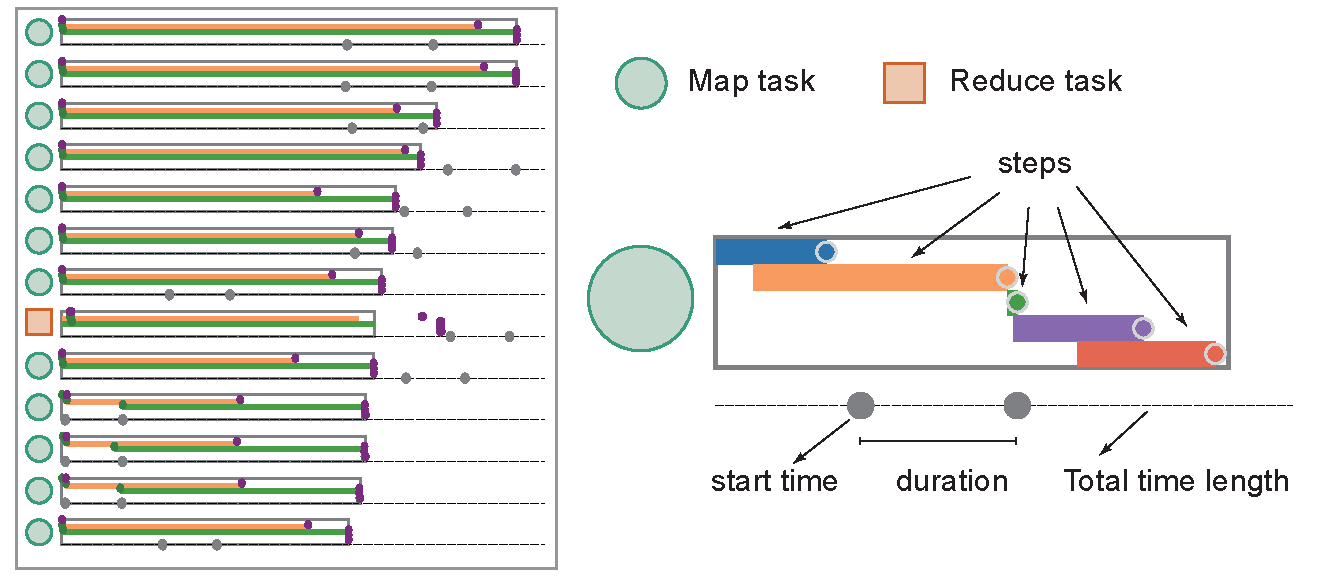
\includegraphics[width=0.48\textwidth]{figures/visualization/taskList.pdf}
	\vspace{-3mm}
	\caption{Visual design for task list.}
	\label{fig:taskList}
	\vspace{-3mm}
\end{figure}

<<<<<<< HEAD
Task list view is developed to enable the detailed exploration of the individual tasks.
All the tasks will be listed from the top to the bottom according to the duration, and only the top one hundred tasks are shown by default.There are two visual forms of a task: glyph form and extension form. By default, the task glyph are placed row by row. When the user select the task of interest, the glyph will be extended as the extension form(shown as ~\ref{**}).


\subsubsection{Task glyph}
As shown by Figure~\ref{fig:taskList}, the green circle or orange rectangle is placed at the left side of a row, indicating the type of the task. On the right side, a rectangle is shown with the length to encode the relative task duration to the maximum duration for all tasks. In the rectangle, the five steps are shown line by line. We use both the color and the y-position to encode the step type. Moreover, the length of a step can be very close to 0, which makes the current visualization unobservable. To tackle this problem, we place a circle and a triangle at the left and right sides of the rectangle of a step, respectively. Thus, the zero-length step will be marked by the overlap of the two shapes.

\subsubsection{Extension View}
When the user clicks the task, an extension view is displayed below to the task glyph, shown as Figure~\ref{fig:taskList}(\textbf{XX}). There are two sub-components in this view: abnormal component and dependency component. 


We first conduct the abnormal detection for the tasks. As suggested by the domain experts, a task is abnormal when its duration is significantly longer than that of other tasks associated with the same vertex and executed on the same machine. Based on these suggestions, we use Tukey Fence~\cite{tukey1977exploratory} to decide if a task is abnormal. With a given set of real integer $S$ and $l \in S$, the anomaly is calculated as follows:

\begin{equation} 
AB(l, S) = \left \{
  \begin{aligned}
    &true, && \text{if}\ l > S.q_3+1.5(S.q_3-S.q_1)\\
    &false, && \text{otherwise}
  \end{aligned} \right.
\end{equation}

Where $S.q_i$ is the $i^{th}$ quartile of set $S$. With the given task and the vertex, we conduct the abnormal detection for the duration of the task and each step. 

After calculation, we design the abnormal component with six rows. With a given vertex $v$ and the task $t$. The top fives row visualize the distribution of the five steps in $v$ as boxplot: the left and right vertical lines indicate the minimum and maximum duration of corresponding steps, and the left and right sides of the rectangle indicate the $1^{st}$ and $3^{st}$ quartiles. We also place a dot over the boxplot to show the duration of task $t$. The last row is implemented to use the same visual form which is used for the presentation of task duration.

The dependency components consists two rows representing the producer tasks and the consumer tasks respectively. With a given task, the number of its consumer tasks and producer tasks may reach thousands of tasks. Considering the scalability issues, we use the pixel barchart~\cite{keim2002pixel} to visualize data amount of dependencies. For example, as shown in Figure~\ref{fig:explorer}{(XX)}, we vertically divide the dependency component into segments to present the machines. 
The consumer tasks or producer tasks are visualized as the pixels in machine box execute this task, the position of task is decided by the data size transmit between the tasks, which is layouted from left to right and from top to bottom. The color is also used to encode the data size. 



%\begin{itemize}
%    \item Our design consideration
%    \item Design: Embedding task view to profiling view
%    \item Design: Visualize the profiling results
%\end{itemize}

\subsection{Interactions}
To facilitate the interactive exploration, out system supports the cross-view interactions. 
In summary, there are two categories of interactions are implemented in the system: cross-level interactions and temporal linkage.

\stitle{Cross-level and -view interactions}:
Our system supports linking among visual elements related to the same task. 
For example, when hovering the mouse on the task of Task View, the corresponding dots of this task and the data dependencies at the machine view will be highlighted by changing the color to purple. Moreover, the progress bar of vertex associated with the task will also be highlighted by change the stroke width.   

\stitle{Temporal linkage}
In both machine view and progress view allow, users can select the time range to narrow down to the pattern of interest. When select time range at any view, the time focus of other views will be updated. 
%    \item Multi-scale navigation
%    \item Inner and inter linking
%\end{itemize}
=======
%Task list view is developed to enable the detailed exploration of the individual tasks.
%All the tasks will be listed from the top to the bottom according to the duration, and only the top one hundred tasks are shown by default.There are two visual forms of a task: glyph form and extension form. By default, the task glyph are placed row by row. When the user select the task of interest, the glyph will be extended as the extension form(shown as ~\ref{**}).

Task View is designed to enable fine-grained exploration of individual tasks.
All tasks are listed from the top to the bottom according to their duration, and only the 150 tasks with the longest duration are shown by default. User can also sort the tasks by There are two visual forms for a task, i.e., glyph form and extension form. By default, the task glyphs are placed row by row. When the user selects a task of interest, its glyph will be extended into the extension form (as shown in Figure~\ref{**}).


\subsubsection{Task Glyph}
As shown in Figure~\ref{fig:taskList}, a green or orange rectangle is placed at the left side of each row to indicate the type of the task. To the right, a rectangle is used to represent a task and its length is proportional to the duration of the task (normalized by the longest task). In a rectangle, the five sub-steps of a task are shown line by line. We use both color and the y-coordinate to encode sub-step types. As the duration of a sub-step can be very close to 0, we place a circle at the left and right sides of the rectangle of a sub-step. Thus, an zero-length sub-step will be marked by the overlap of the two shapes.

\subsubsection{Extension View}
%When the user clicks the task, an extension view is displayed below to the task glyph, shown as Figure~\ref{fig:taskList}(\textbf{XX}). There are two sub-components in this view: abnormal component and dependency component. 
%
%
%We first conduct the abnormal detection for the tasks. As suggested by the domain experts, a task is abnormal when its duration is significantly longer than that of other tasks associated with the same vertex and executed on the same machine. Based on these suggestions, we use Tukey Fence~\cite{tukey1977exploratory} to decide if a task is abnormal. With a given set of real integer $S$ and $l \in S$, the anomaly is calculated as follows:
%
%\begin{equation} 
%AB(l, S) = \left \{
%  \begin{aligned}
%    &true, && \text{if}\ l > S.q_3+1.5(S.q_3-S.q_1)\\
%    &false, && \text{otherwise}
%  \end{aligned} \right.
%\end{equation}
%
%Where $S.q_i$ is the $i^{th}$ quartile of set $S$. With the given task and the vertex, we conduct the abnormal detection for the duration of the task and each step. 
%
%After calculation, we design the abnormal component with six rows. With a given vertex $v$ and the task $t$. The top fives row visualize the distribution of the five steps in $v$ as boxplot: the left and right vertical lines indicate the minimum and maximum duration of corresponding steps, and the left and right sides of the rectangle indicate the $1^{st}$ and $3^{st}$ quartiles. We also place a dot over the boxplot to show the duration of task $t$. The last row is implemented to use the same visual form which is used for the presentation of task duration.
%
%The dependency components consists two rows representing the producer tasks and the consumer tasks respectively. With a given task, the number of its consumer tasks and producer tasks may reach thousands of tasks. Considering the scalability issues, we use the pixel barchart~\cite{keim2002pixel} to visualize data amount of dependencies. For example, as shown in Figure~\ref{fig:explorer}, we vertically divide the dependency component into segments to present the machines. 
%The consumer tasks or producer tasks are visualized as the pixels in machine box executing this task, the position of task is decided by the data size transmit between the tasks, which is layouted from left to right and from top to bottom. The color is also used to encode the data size. 



%\begin{itemize}
%    \item Our design consideration
%    \item Design: Embedding task view to profiling view
%    \item Design: Visualize the profiling results
%\end{itemize}




When the user clicks a task, an extension view is displayed below the task glyph as shown in Figure~\ref{fig:taskList}(\textbf{XX}). The extension view contains two components, i.e., abnormal view and dependency component. 

In the abnormal view, we conduct anomaly detection for the tasks. As suggested by the domain experts, a task is likely to be abnormal if its duration is significantly longer than that other tasks that correspond to the same vertex in the logical DAG and run on the same machine. Based on this suggestion, we use the Tukey Fence method~\cite{tukey1977exploratory} to decide if a task is abnormal. For a set of real numbers $S$ and a number $l \in S$, the anomaly score of $l$ calculated as

\begin{equation} 
	AB(l, S) = \left \{
	\begin{aligned}
		&true, && \text{if}\ l > S.q_3+1.5\times(S.q_3-S.q_1)\\
		&false, && \text{otherwise}
	\end{aligned} \right.,
\end{equation}

where $S.q_i$ is the $i^{th}$ quartile of set $S$. Given a task and its corresponding logical vertex, we calculate the anomaly score for both the task a whole and its 5 sub-steps. With the anomaly score, we use six rows in the abnormal component. For a task $t$ and its vertex $v$, the top five rows visualize the duration distribution of the five sub-steps in $v$ using box plot: the left and right vertical lines indicate the minimum and maximum duration of the corresponding sub-steps, and the left and right sides of the rectangle indicate the $1^{st}$ and $3^{st}$ quartile. We also place a dot over the box plot to show the duration of task $t$. The last row use the same visual as for task duration.

The dependency view consists two rows representing the producer tasks and consumer tasks that are related to the selected task, respectively. As the number of consumer tasks and producer tasks can reach thousands, we use the pixel bar chart~\cite{keim2002pixel} due to scalability issues. As shown in Figure~\ref{fig:explorer}, we vertically divide the dependency view into segments to represent different machines. 
The consumer tasks or producer tasks are visualized as pixels in the boxes corresponding to machines that execute this task. The position of a dependent task is decided by the data size transmitted between it and the selected task. The dependent tasks are placed from left to right in descending order of their data transfer and color encoding (from dark red to light yellow) is also used to indicate the data size. 

\subsection{Interactions}
%To facilitate interactive exploration, out system supports the cross-view interactions. 
%In summary, there are two categories of interactions are implemented in the system: cross-level interactions and temporal linkage.
%
%\stitle{Cross-level and -view interactions}
%Our system supports linking among visual elements related to the same task. 
%For example, when hovering the mouse on the task of Task View, the corresponding dots of this task and the data dependencies at the machine view will be highlighted by changing the color to purple. Moreover, the progress bar of vertex associated with the task will also be highlighted by change the stroke width.   
%
%\stitle{Temporal linkage}
%In both machine view and progress view allow, users can select the time range to narrow down to the pattern of interest. When select time range at any view, the time focus of other views will be updated. 


To facilitate interactive exploration, $\DQV$ supports two types of cross-view interactions, i.e., cross-level interaction and temporal linkage.

\stitle{Cross-level and cross-view interaction}
$\DQV$ supports linking visual elements related to the same task. 
For example, if the user hovers the mouse on one task in the task view, the dot that corresponds to the task and its data dependencies of on the machine view will be highlighted by changing the color to purple. Moreover, the progress bar of the logical vertex associated with the task will be highlighted by changing the stroke width.   

\stitle{Temporal linkage}
In both machine view and progress view, the user can select the time range to narrow down the focus of interest. If time range is selected in one view, other views will adjust their time ranges accordingly.

>>>>>>> 87e38476d46c232532b1981a1ff0ea0f46d2299d
